\documentclass{article}

\usepackage[preprint, nonatbib]{neurips_2021}
\usepackage[utf8]{inputenc} % allow utf-8 input
\usepackage[T1]{fontenc}    % use 8-bit T1 fonts
\usepackage{hyperref}       % hyperlinks
\usepackage{url}            % simple URL typesetting
\usepackage{booktabs}       % professional-quality tables
\usepackage{amsfonts}       % blackboard math symbols
\usepackage{nicefrac}       % compact symbols for 1/2, etc.
\usepackage{microtype}      % microtypography
\usepackage{xcolor}         % colors
\usepackage{graphicx}
\usepackage{caption}
\usepackage{subcaption}
\usepackage[
backend=biber,
style=numeric,
citestyle=ieee
]{biblatex}
\addbibresource{references.bib} %Imports bibliography file

\title{YouTube Trending Video Analysis\\
for Germany\thanks{The source files are available at \url{https://github.com/lgehring/yt_trends}}}

\author{%
  L. Gehring \\
  Matriculation number XXXXXXX\\
  University of Tübingen\\
  \texttt{l.gehring@student.uni-tuebingen.de} \\
}

\begin{document}

\maketitle

\begin{abstract}
  The content and some appealing metrics of the YouTube Trending category are laid out
  in the context of YouTube's own ideals. Further, the paper infers, 
  why the category might not be representative of actual trends on the YouTube platform.
\end{abstract}

\section{What is \textit{Trending on YouTube}?}
YouTube Trending is a non-personalized subpage on the YouTube website, that showcases 50 algorithmically selected videos at all times. The selection of videos gets updated roughly every 15 minutes. Although the exact selection algorithm is kept secret, YouTube states, that the videos presented `aim(s) to surface videos that a wide range of viewers would find interesting.'

Further, they list some specific favorable video properties, e.g. `appealing to a wide range of viewers', `not misleading, clickbaity or sensational', and `ideally, (are) surprising or novel'. To quantify the stated criteria, YouTube claims to (but not only) utilize view count, view count increase speed, age of the video and intra-channel performance comparisons \cite{trends_help}.

In order to gain insight into the workings of YouTube Trending and to compare reality to YouTube's stated ideals, some data from the `YouTube Trending Video Dataset' \cite{data} was evaluated.

The dataset contains daily entries of the videos currently listed in trending alongside their corresponding metadata, e.g. upload-time, (dis-)likes, channel name, title, tags and category. The entries start 12/08/2020 and up to time of writing (last update: 03/02/2022) are updated daily.

\section{\textit{What} is trending on YouTube?}
\begin{figure}[h]
    \centering
    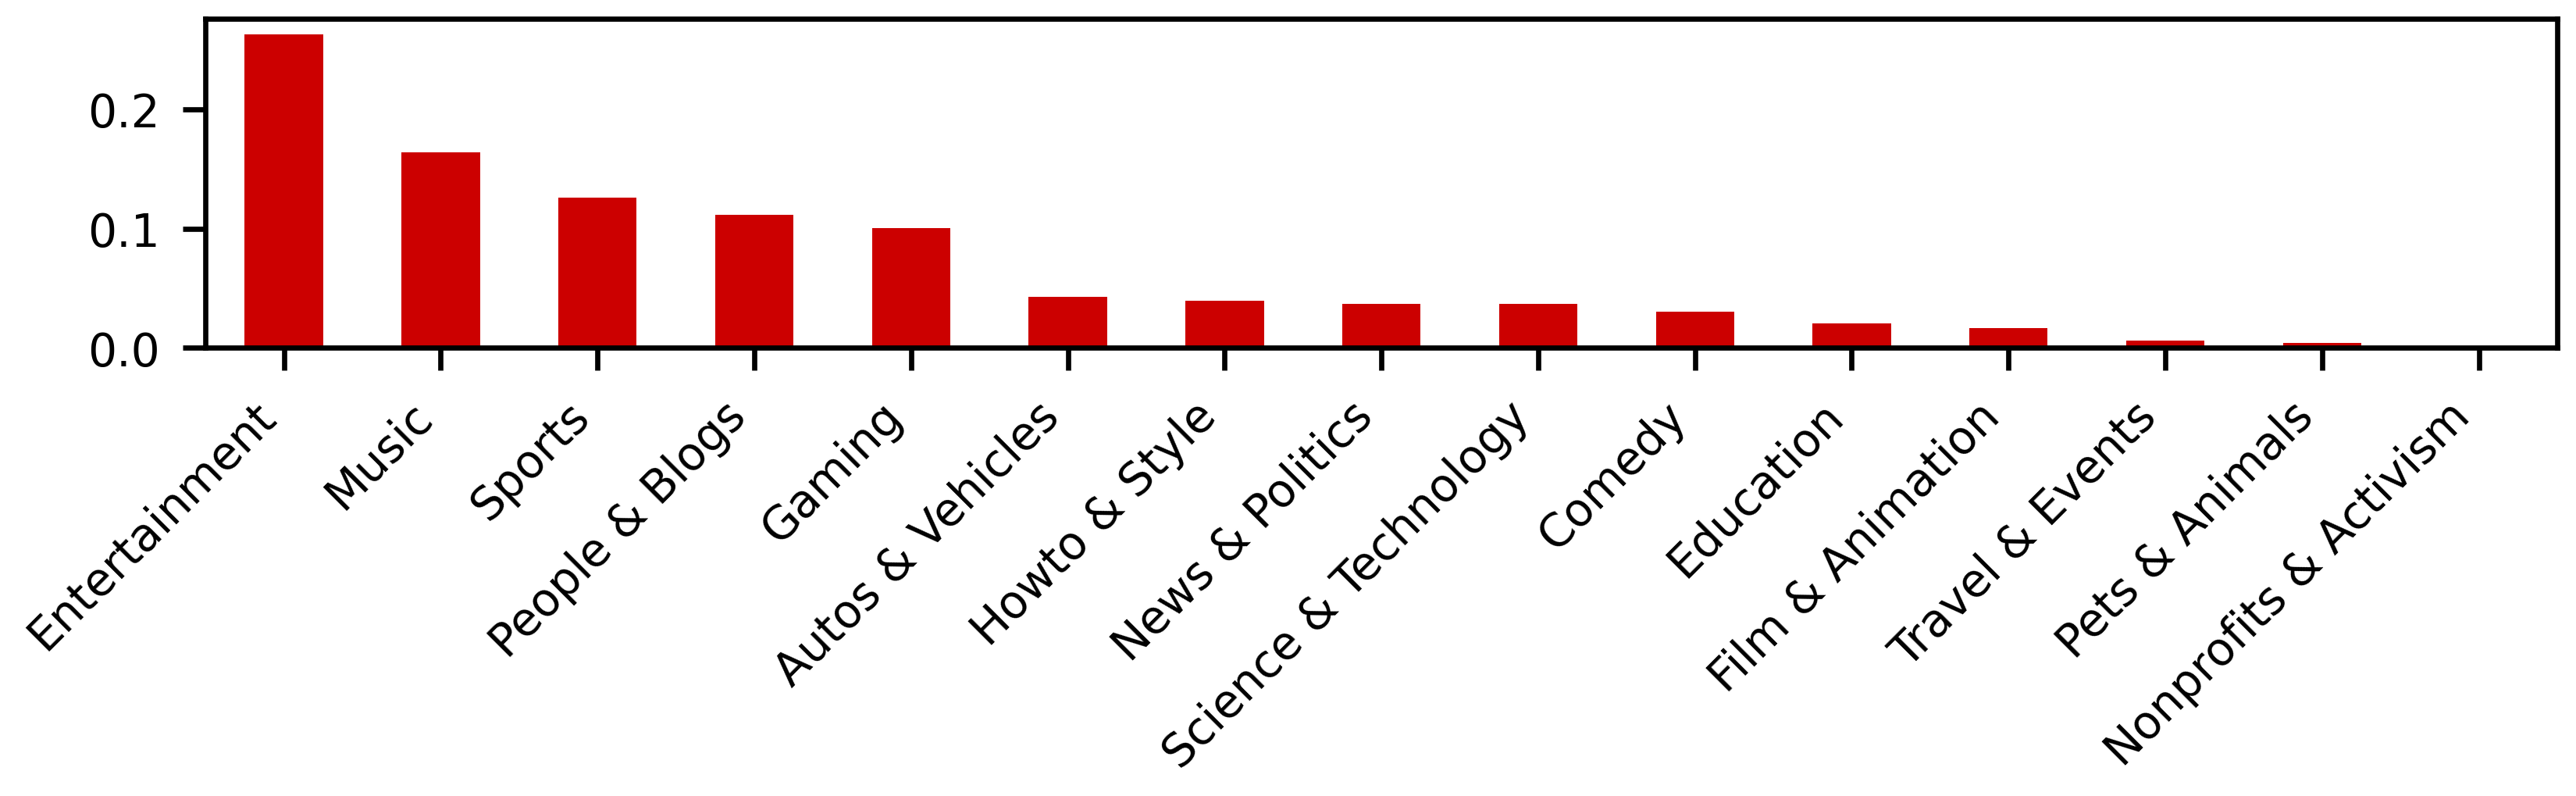
\includegraphics[width=0.8\textwidth]{fig/pop_cat.png}
    \caption{Popular video categories by relative share}
    \label{fig:pop_cat}
\end{figure}

\paragraph{Categories} The dataset used enables the investigation of popularity in several dimensions. One of which would be to simply compare the share of the trending videos assigned categories. A category is automatically assigned to the video upon upload, unless the uploader overrides this decision.

As the algorithm allegedly does not factor video category into the ranking metric \cite{cat_legacy}, the category distribution (Fig. \ref{fig:pop_cat}) should give a broad impression of what type of content is generally watched on the platform.

Roughly a quarter of all trends fall into the `Entertainment' category, and about one-sixth of videos are `Music'. The runners-up are `Sports', `People \& Blogs' and `Gaming', all in the $\sim$10-13\% range. 

All five together account for round about three-quarters of videos in trending.

\begin{figure}[h]
    \centering
    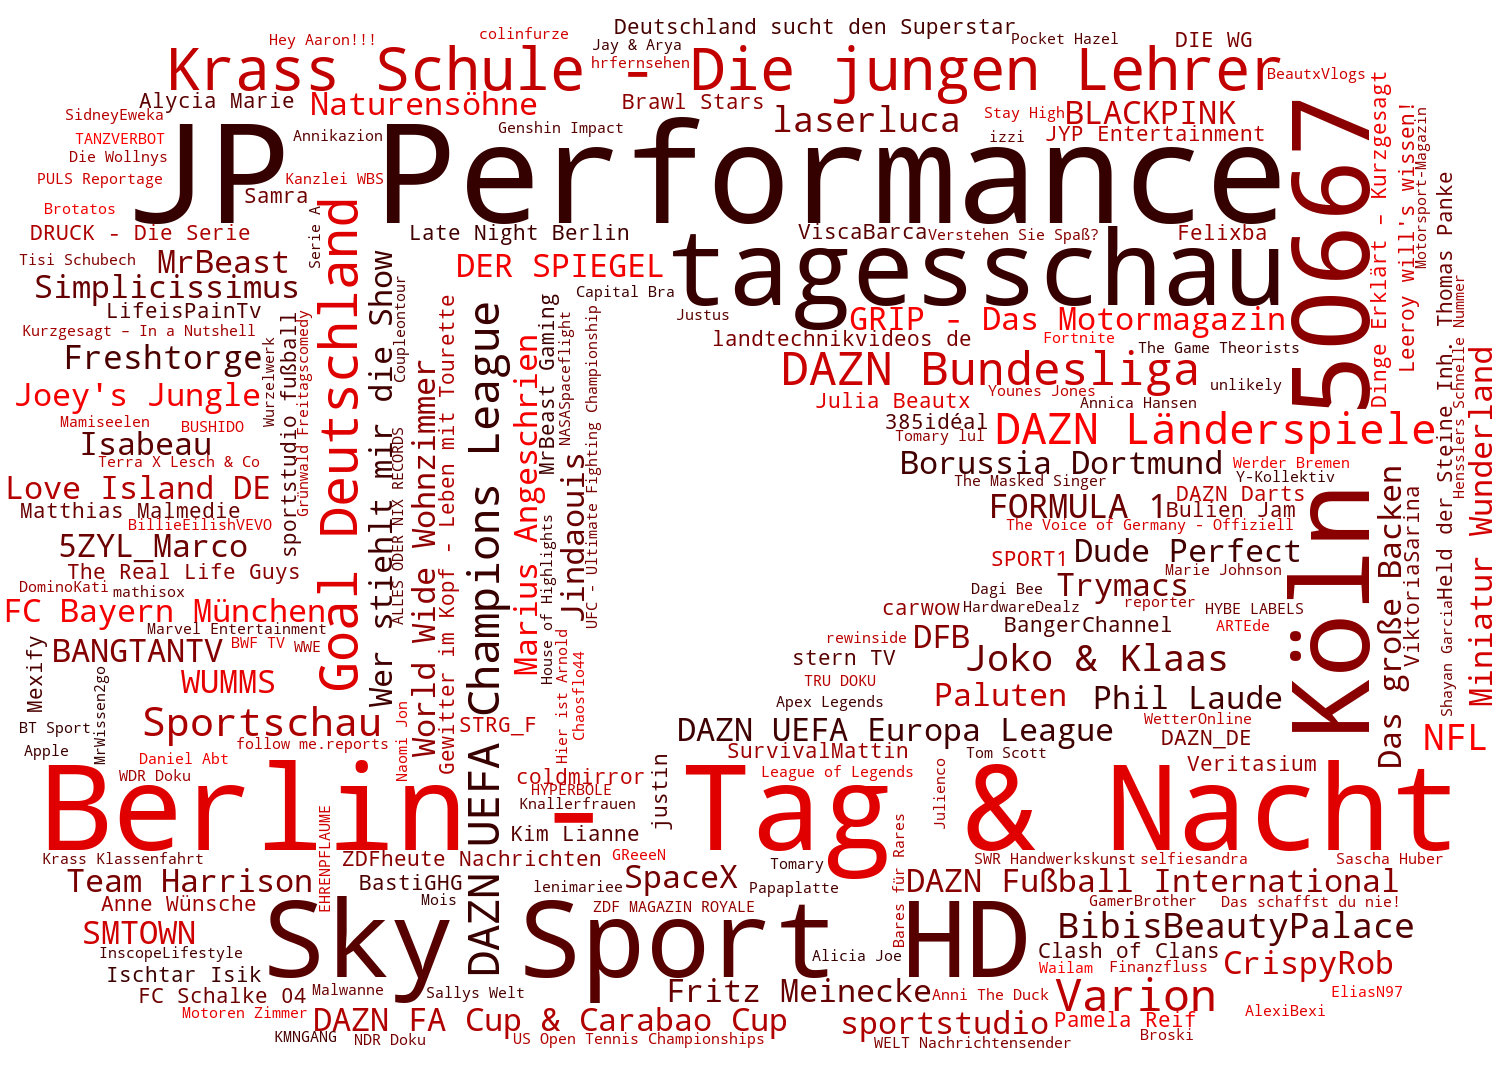
\includegraphics[width=0.625\textwidth]{fig/channels_wordcloud_nice.png}
    \caption{Trending channels as 'YouTube logo word cloud'}
    \label{fig:wc_channels}
\end{figure}

\paragraph{Channels, Tags and Titles} Another dimension to explore, is the frequency, with which videos from certain channels appear in the trending tab. For this, the font-size in Fig. \ref{fig:wc_channels} was adjusted to the frequency of appearance.

Six channels stand out from the cloud: `JP Performance', `Berlin - Tag \& Nacht', `Sky Sport HD', `Köln 50667', `tagesschau' and `Krass Schule - Die jungen Lehrer'. Interestingly, all big players except the first mentioned are regular German TV show formats. Additionally, there are 12 channels hosted by the sports streaming service `DAZN', that together hold more than twice the share of `JP Performance' (0.92\% vs. 2.06\%).

In similar fashion, popular tags (Fig. \ref{fig:wc_tags}) and words used in the title (Fig. \ref{fig:wc_titles}) can be examined. Some of the most frequent tags are: `RTL', `deutsch', `funny', `lustig', `comedy', `vlog', and `DAZN'. Notable popular words (with character count $\geq 4$ ) used in the title are: `Official', `Video', `Highlights', `2021', `DAZN' and `\#shorts'. The latter is used to mark short-form videos, similar to `TikTok' in style \cite{shorts_help}, while `Official Video' is often used in titles of music videos.

\paragraph{Thumbnails} One more approach to gain insight into the content promoted by YouTube Trending, is to look at the thumbnails (= miniature preview pictures) of the videos. As the interest lies on the general trend of imagery, a general impression may be obtained by averaging over all thumbnails. For this, the mean value for each pixel was computed over all videos (3.5\% of videos were ignored due to broken download links). The result can be seen in Fig. \ref{fig:avg_thumbnail}. 

A vertical light bar is visible, which is likely caused by videos filmed vertically with a smartphone (probably mostly \#shorts). The black bars atop and on the bottom are a result of the necessity to accommodate for vertical and horizontal videos in the same format. 

The general hue of the picture is a pale skin tone, with darker edges and corners. This \textit{might be} a result of the very frequent appearance of light skinned faces in the thumbnails. In the top left corner, a white square with the `DAZN' logo is dominant. In the bottom left corner, the `vevo' logo (a music video network), as well as a yellowish on black score counter, are visible.

\begin{figure}[ht]
    \centering
    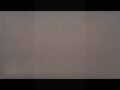
\includegraphics[width=0.5\textwidth]{fig/average_thumbnail.png}
    \caption{Artificial `average thumbnail'}
    \label{fig:avg_thumbnail}
\end{figure}

\section{How is trending content produced and consumed?}
\paragraph{Durations} The average trending video gets classified as such $1.4 \pm 1.6$ days after release (onset duration) and stays in trending for $4.2 \pm 1.3$ days on average (trending duration). The maximum onset duration was 32 days and the max. trending duration 10 days. Time of upload was ignored for this computation, because the provided trending timestamps have only a one-day resolution.

\begin{figure}[h]
    \centering
    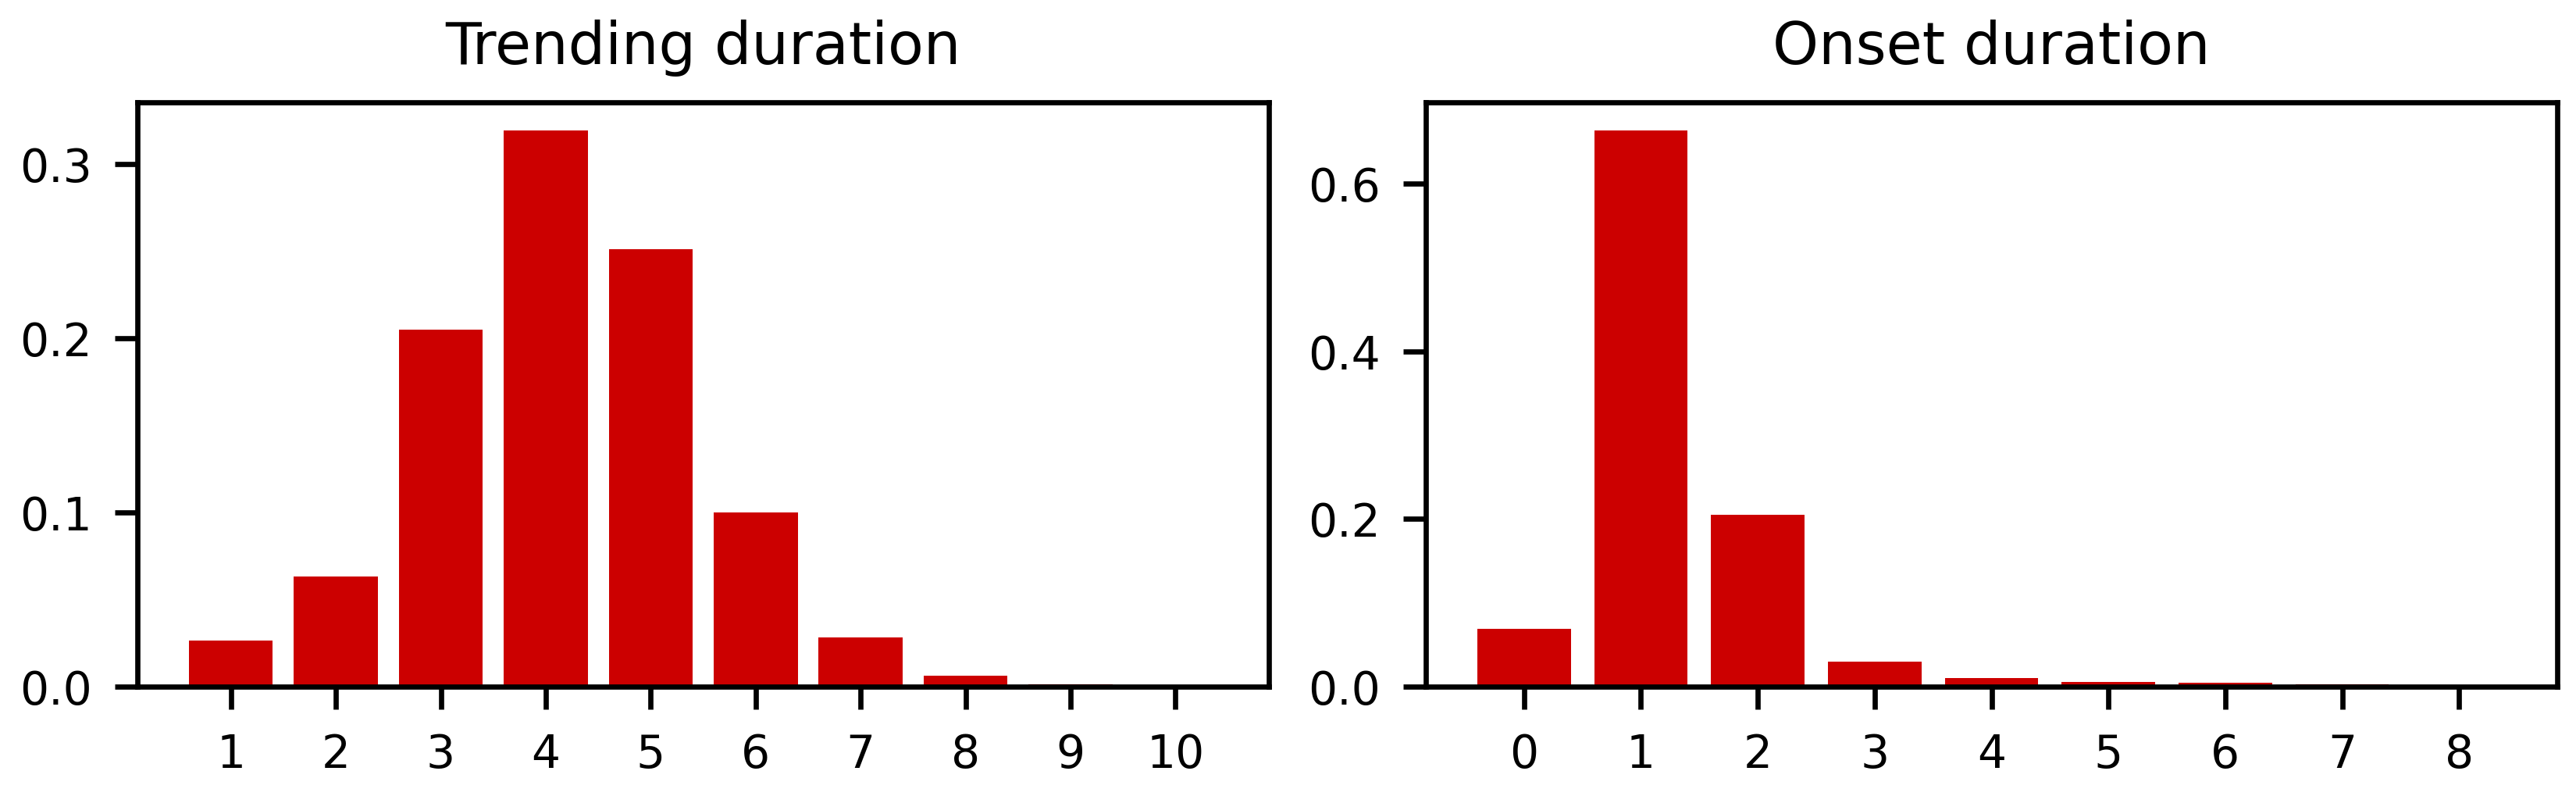
\includegraphics[width=0.8\textwidth]{fig/durations.png}
    \caption{Trending and onset duration distributions (in days)}
    \label{fig:durations}
\end{figure}

\paragraph{Production} Considering the upload times (with hourly resolution), some clear time windows are revealed (Fig. \ref{fig:pub_time}). Throughout the week, the afternoon from 15 to 18 o'clock appears to be a general trend for video releases. The most popular days are Monday through Thursday and Sunday, with Wednesday being the most frequent option. 

Three anomalous publishing times are Thursday night from 22 to 24 o'clock (caused by `DAZN UEFA Europa League'), Sunday 9 to 11 o'clock (`BibisBeautyPalace', `Joey's Jungle', `Phil Laude', `Julia Beautx') and Friday morning between 4 and 6 o'clock (`ABC').

\begin{figure}[h]
    \centering
    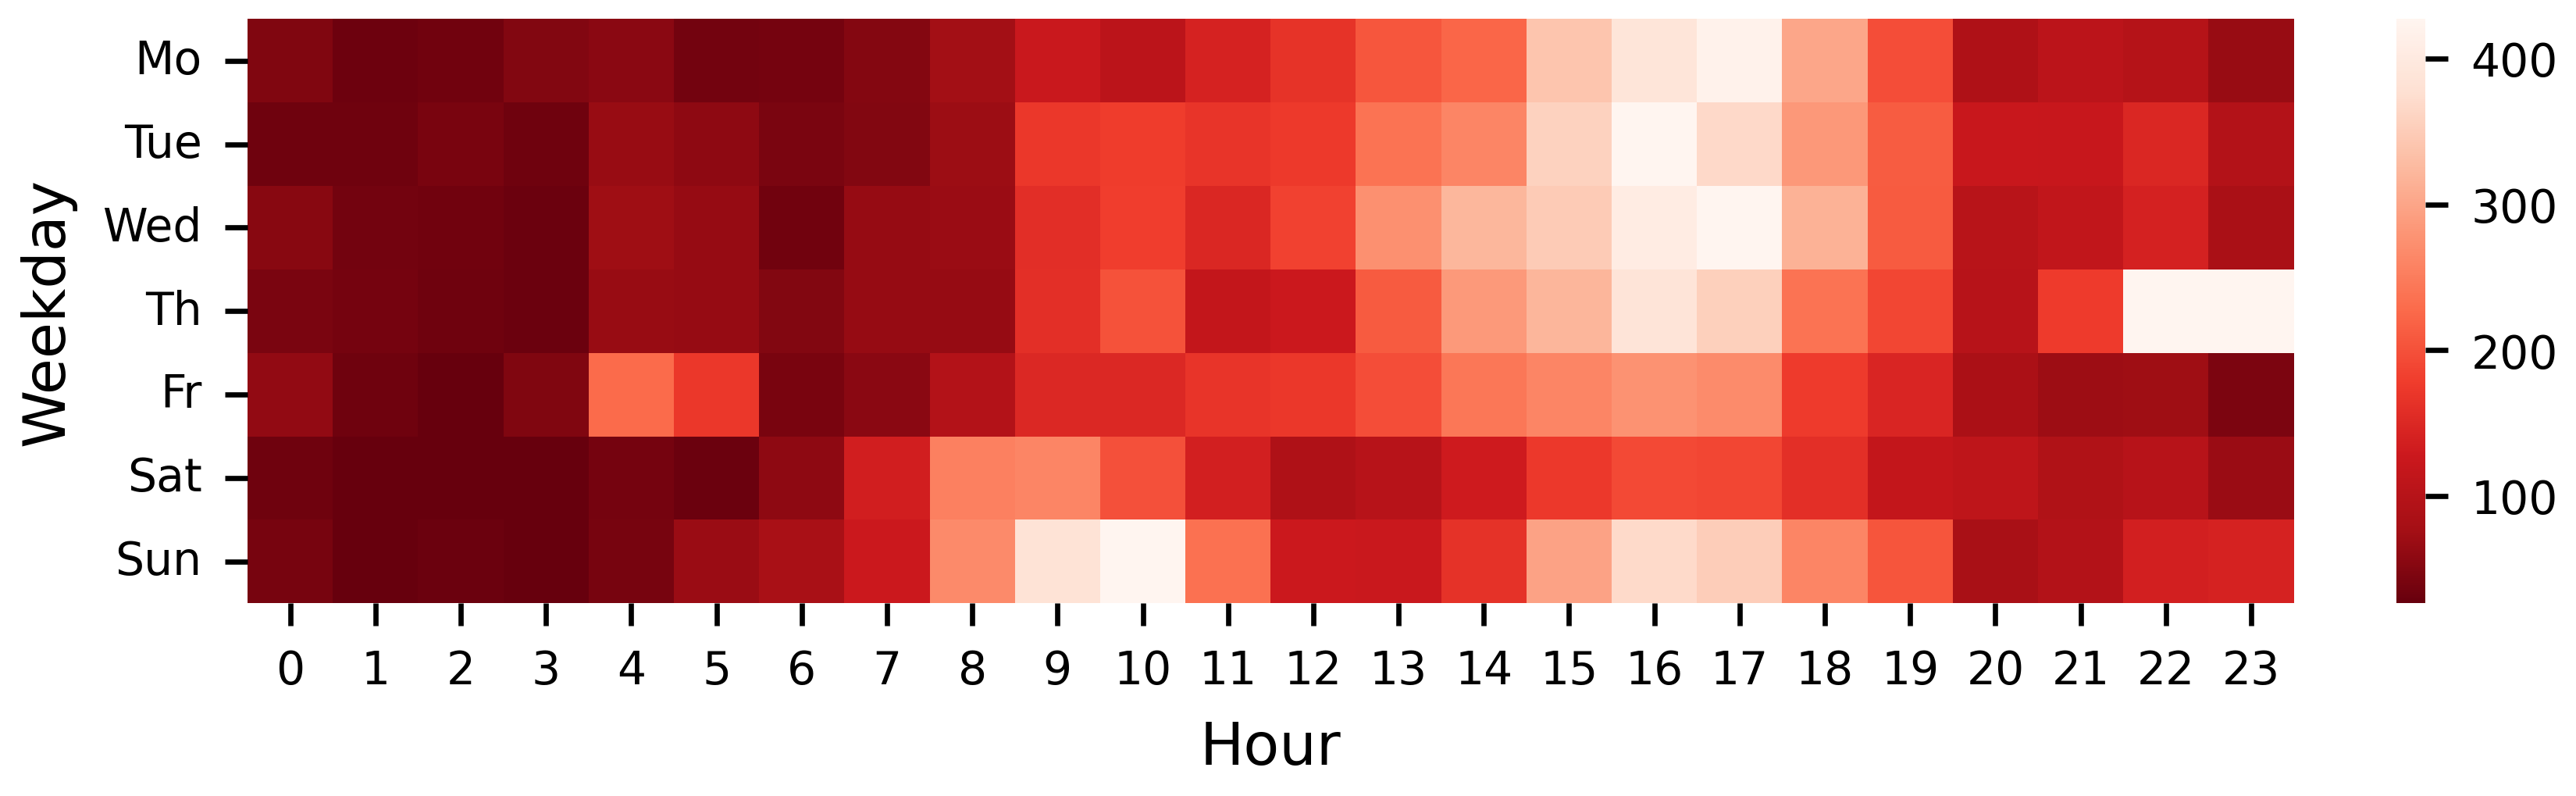
\includegraphics[width=\textwidth]{fig/pub_time.png}
    \caption{Publication times of trending videos (in no. of videos)}
    \label{fig:pub_time}
\end{figure}

\begin{figure}[ht]
    \centering
    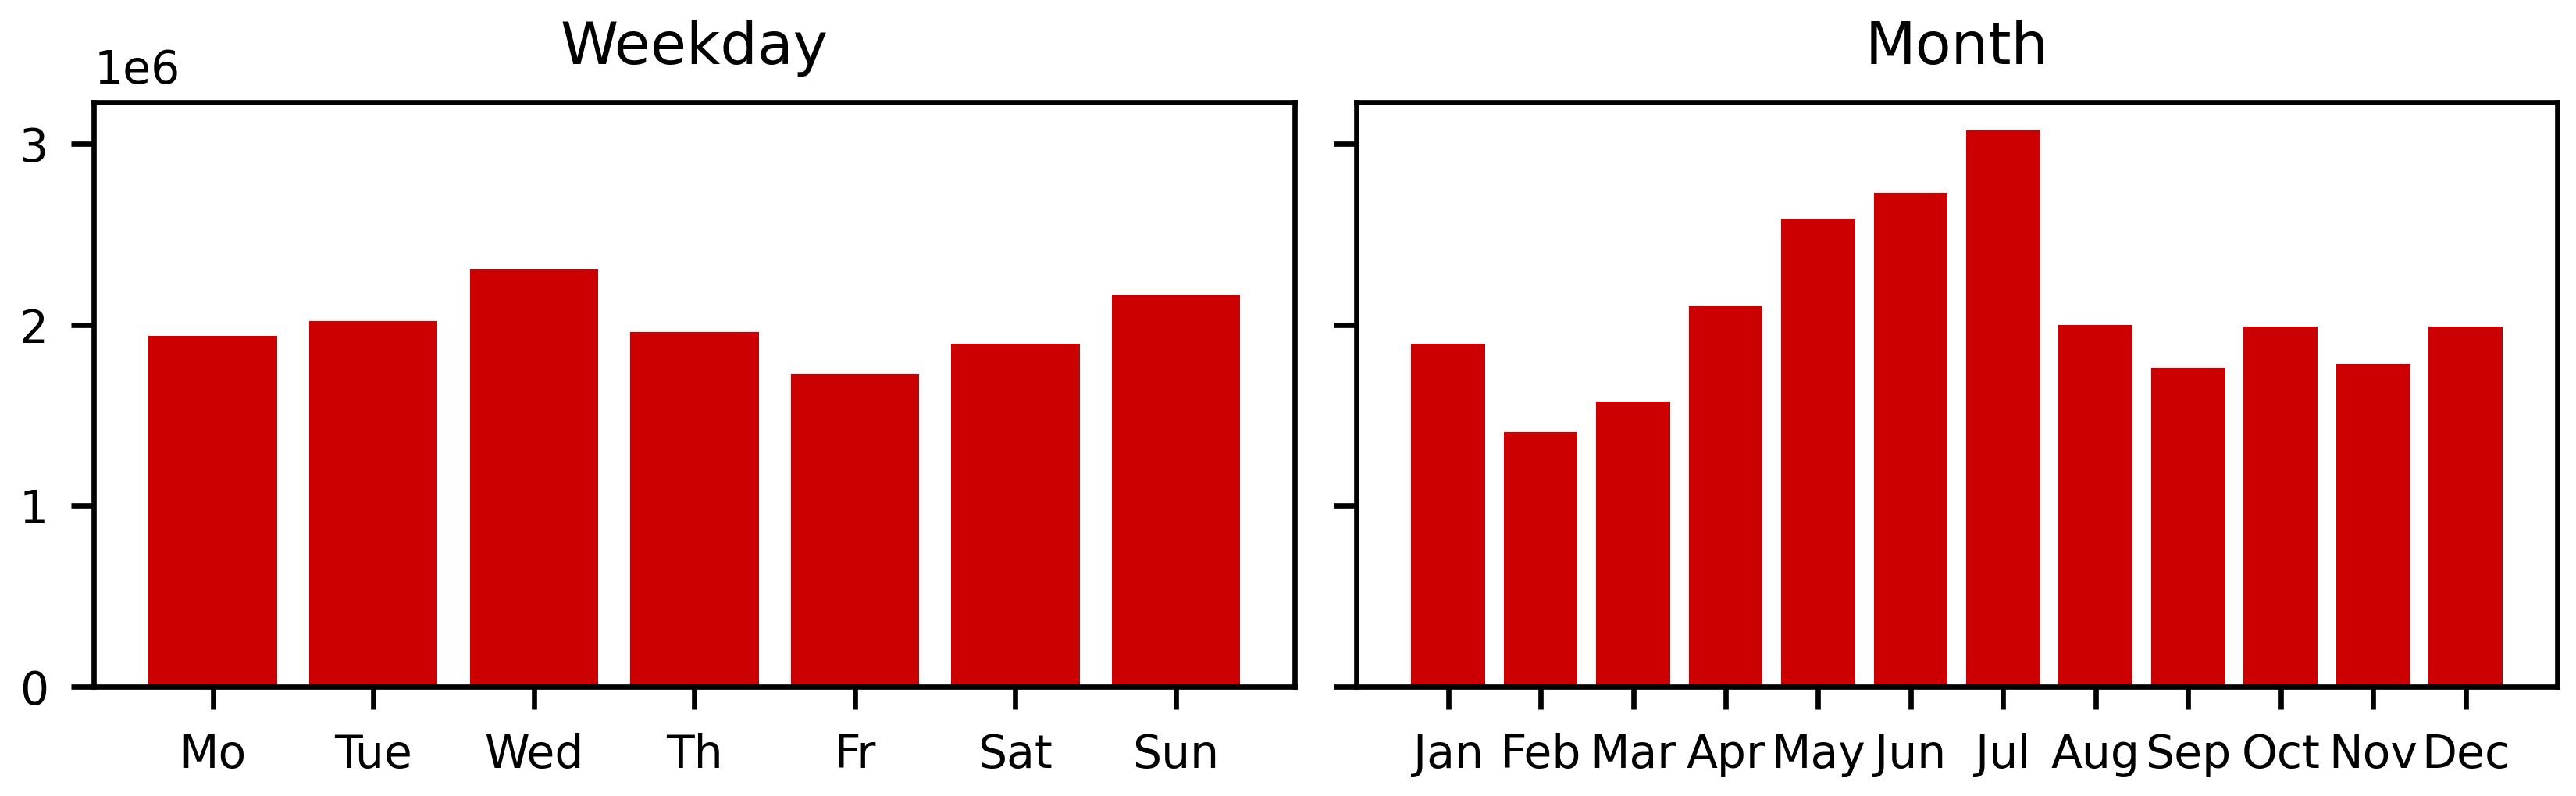
\includegraphics[width=0.8\textwidth]{fig/views.png}
    \caption{Average views per video and weekday/month}
    \label{fig:views}
\end{figure}

\paragraph{Consumption} The average `performance' of videos heavily fluctuates over time (Fig. \ref{fig:views}). During the course of a week, Wednesday and Sunday record the highest engagement measured by views, while Friday is last. Those trends are in accordance with the upload times from Fig. \ref{fig:pub_time}, which \textit{could} be hinting at e.g. active planning of upload times. This is pure speculation.

Contrary to the initial expectations, the number of views during the late spring and early summer (May - Jul) is higher than all other months. February presents the least no. of views per video. The remaining months are relatively consistent in view counts.

\paragraph{Additional Characteristics} An assessment of inter-feature Pearson correlations (Tab. \ref{tab:corr_tab}) reveals three noteworthy traits. Most prominent, the no. of comments are positively correlated with the no. of likes (0.29) and dislikes (0.19). Also, the number of views seems to have a positive relation to the onset duration (0.2). A mild positive correlation exists between views and trending duration (0.13). Lastly, a mild negative parallel can be found amid onset and trending duration (-0.12).

\begin{table}[h]
    \centering
    \caption{Correlations}
    \resizebox{0.875\textwidth}{!}{
        \begin{tabular}{lrrrrrr}
\toprule
{} &  views &  likes &  dislikes &  comments &  trending duration &  onset duration \\
\midrule
views             &   1.00 &  -0.03 &     -0.02 &     -0.02 &               0.13 &            0.20 \\
likes             &        &   1.00 &      0.02 &      0.29 &              -0.00 &           -0.05 \\
dislikes          &        &        &      1.00 &      0.19 &               0.01 &            0.01 \\
comments          &        &        &           &      1.00 &              -0.01 &           -0.07 \\
trending duration &        &        &           &           &               1.00 &           -0.12 \\
onset duration    &        &        &           &           &                    &            1.00 \\
\bottomrule
\end{tabular}

    }
    \label{tab:corr_tab}
\end{table}

\section{Does YouTube Trending keep its promise?}
Above, a wide range of characteristics were presented, many of which do not support the claim of highlighting ‘videos that a wide range of viewers would find interesting’. The categories most frequent represented and the channels mainly serving that content show many properties of `old school TV' combined with that of a music video network. YouTube \#shorts is the only popular tag remotely original to YouTube-style content. 

In terms of flexibility, YouTube Trends are theoretically capable of quickly adapting to current trends with short onset and trending durations, but they are prone to featuring the same type of content like sports highlights and TV series episodes over and over again, practically failing at least one declared goal of selecting videos that are ‘surprising or novel'.

\printbibliography

\newpage
\appendix
\section{Appendix}
\begin{figure}[h]
\centering
\begin{subfigure}{.5\textwidth}
    \centering
    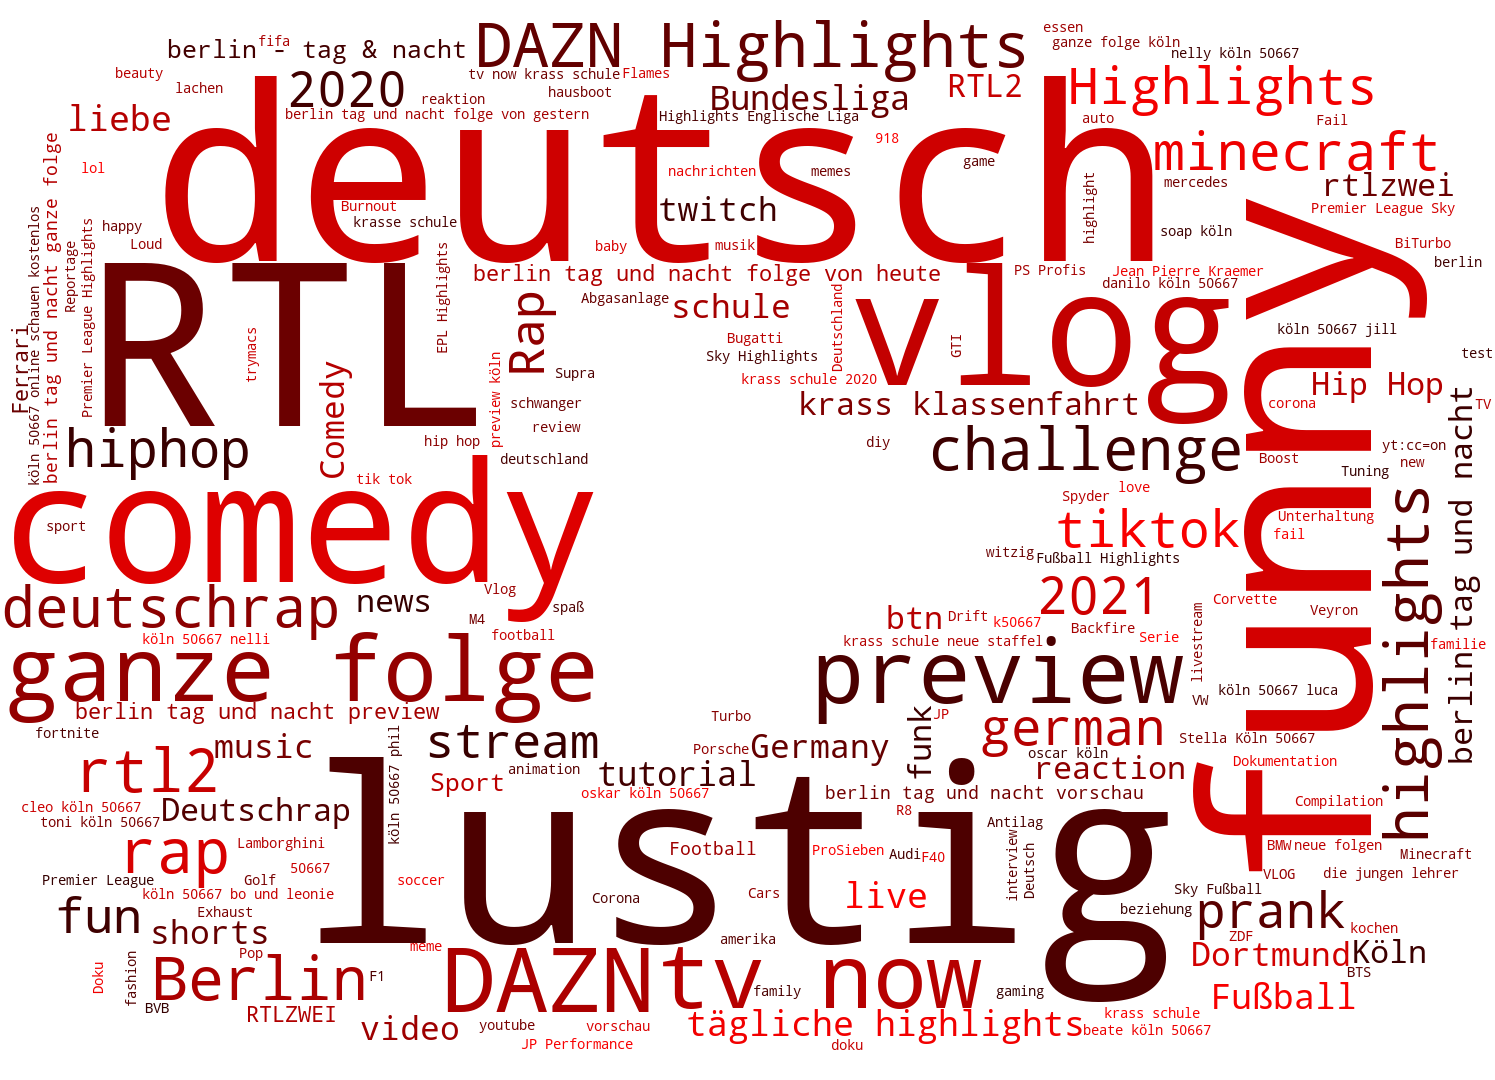
\includegraphics[width=0.75\textwidth]{fig/tags_wordcloud_nice.png}
    \caption{Trending tags as 'YouTube logo word cloud'}
    \label{fig:wc_tags}
\end{subfigure}%
\begin{subfigure}{.5\textwidth}
    \centering
    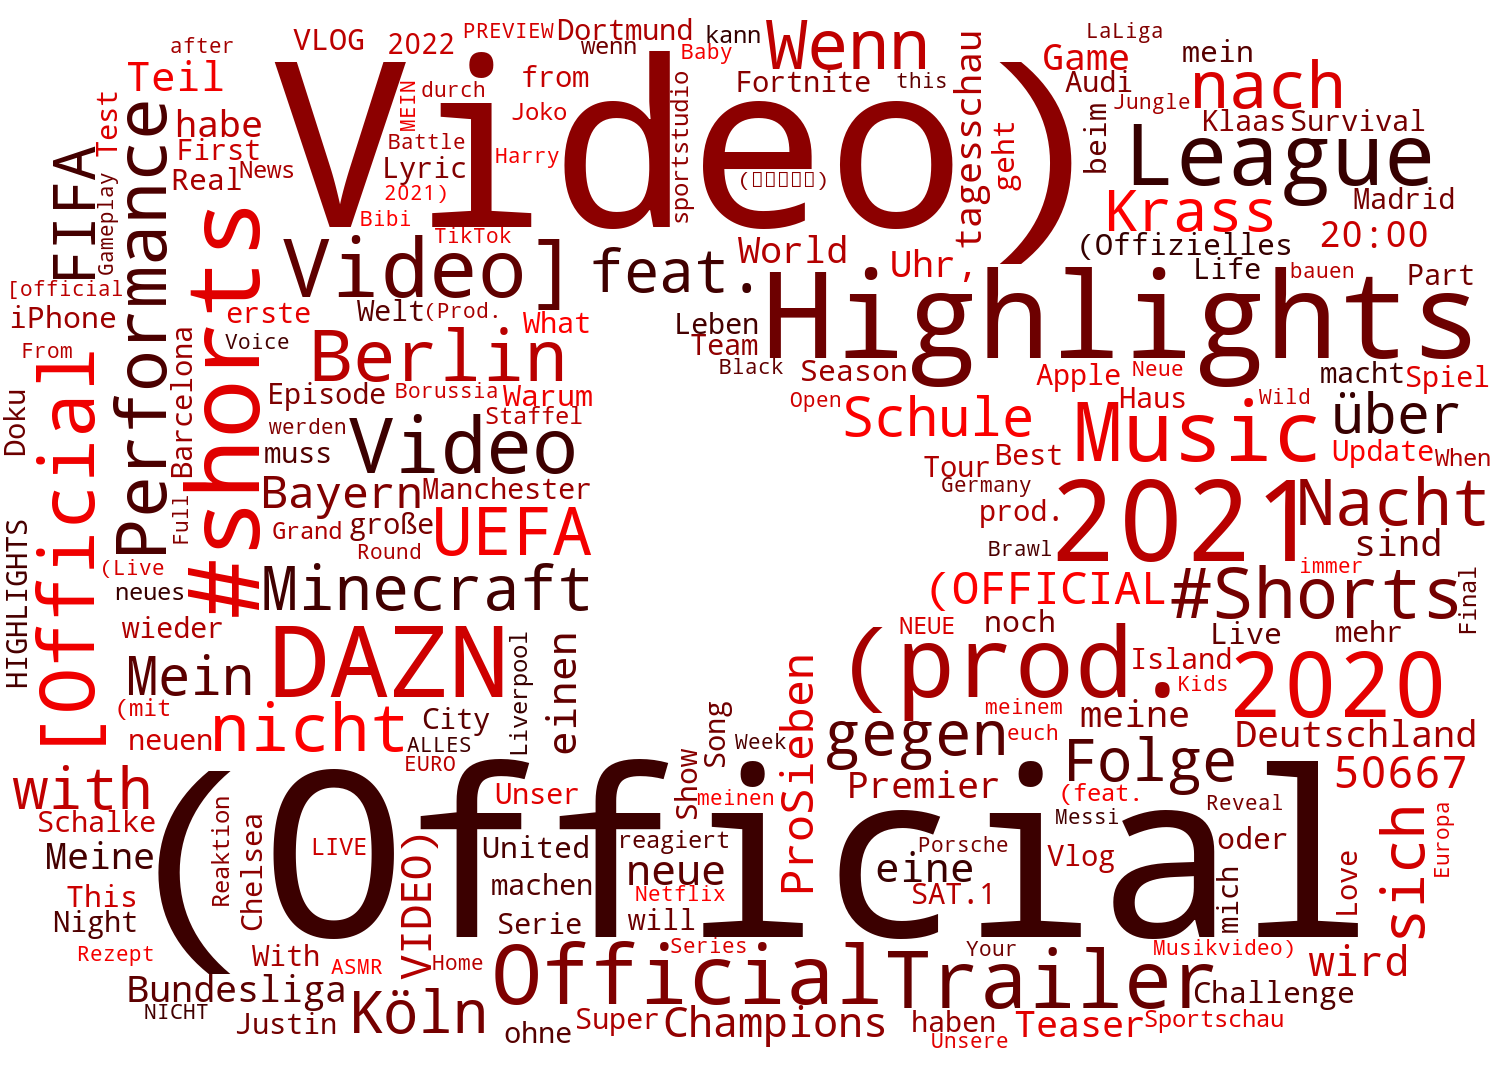
\includegraphics[width=0.75\textwidth]{fig/titles_wordcloud_nice.png}
    \caption{Trending title words as 'YouTube logo word cloud'}
    \label{fig:wc_titles}
\end{subfigure}
\caption{Additional word clouds}
\label{fig:wc_appendix}
\end{figure}

An additional aspect to explore, is the share each category holds over the course of a week or year, which can be seen in Fig. \ref{fig:cat_cycle}. 

It can be observed, that `Music' videos tend to trend in the first half of the week, while the `Entertainment' share rises towards the weekend. Also, `Howto \& Style' and `Sports' both peak on Thursdays. It is notable, that the `Entertainment' category steadily declines in popularity between March and September, but generally gains momentum in the opposite half of the year. Interest in `Gaming' seems to drop during February and March. `Sports' gained attention in August. 

As the data stems from a timespan smaller than two years (Aug 20 - Jan 22), especially the monthly popularity estimates should be taken with a grain of salt.

\begin{figure}[h]
    \centering
    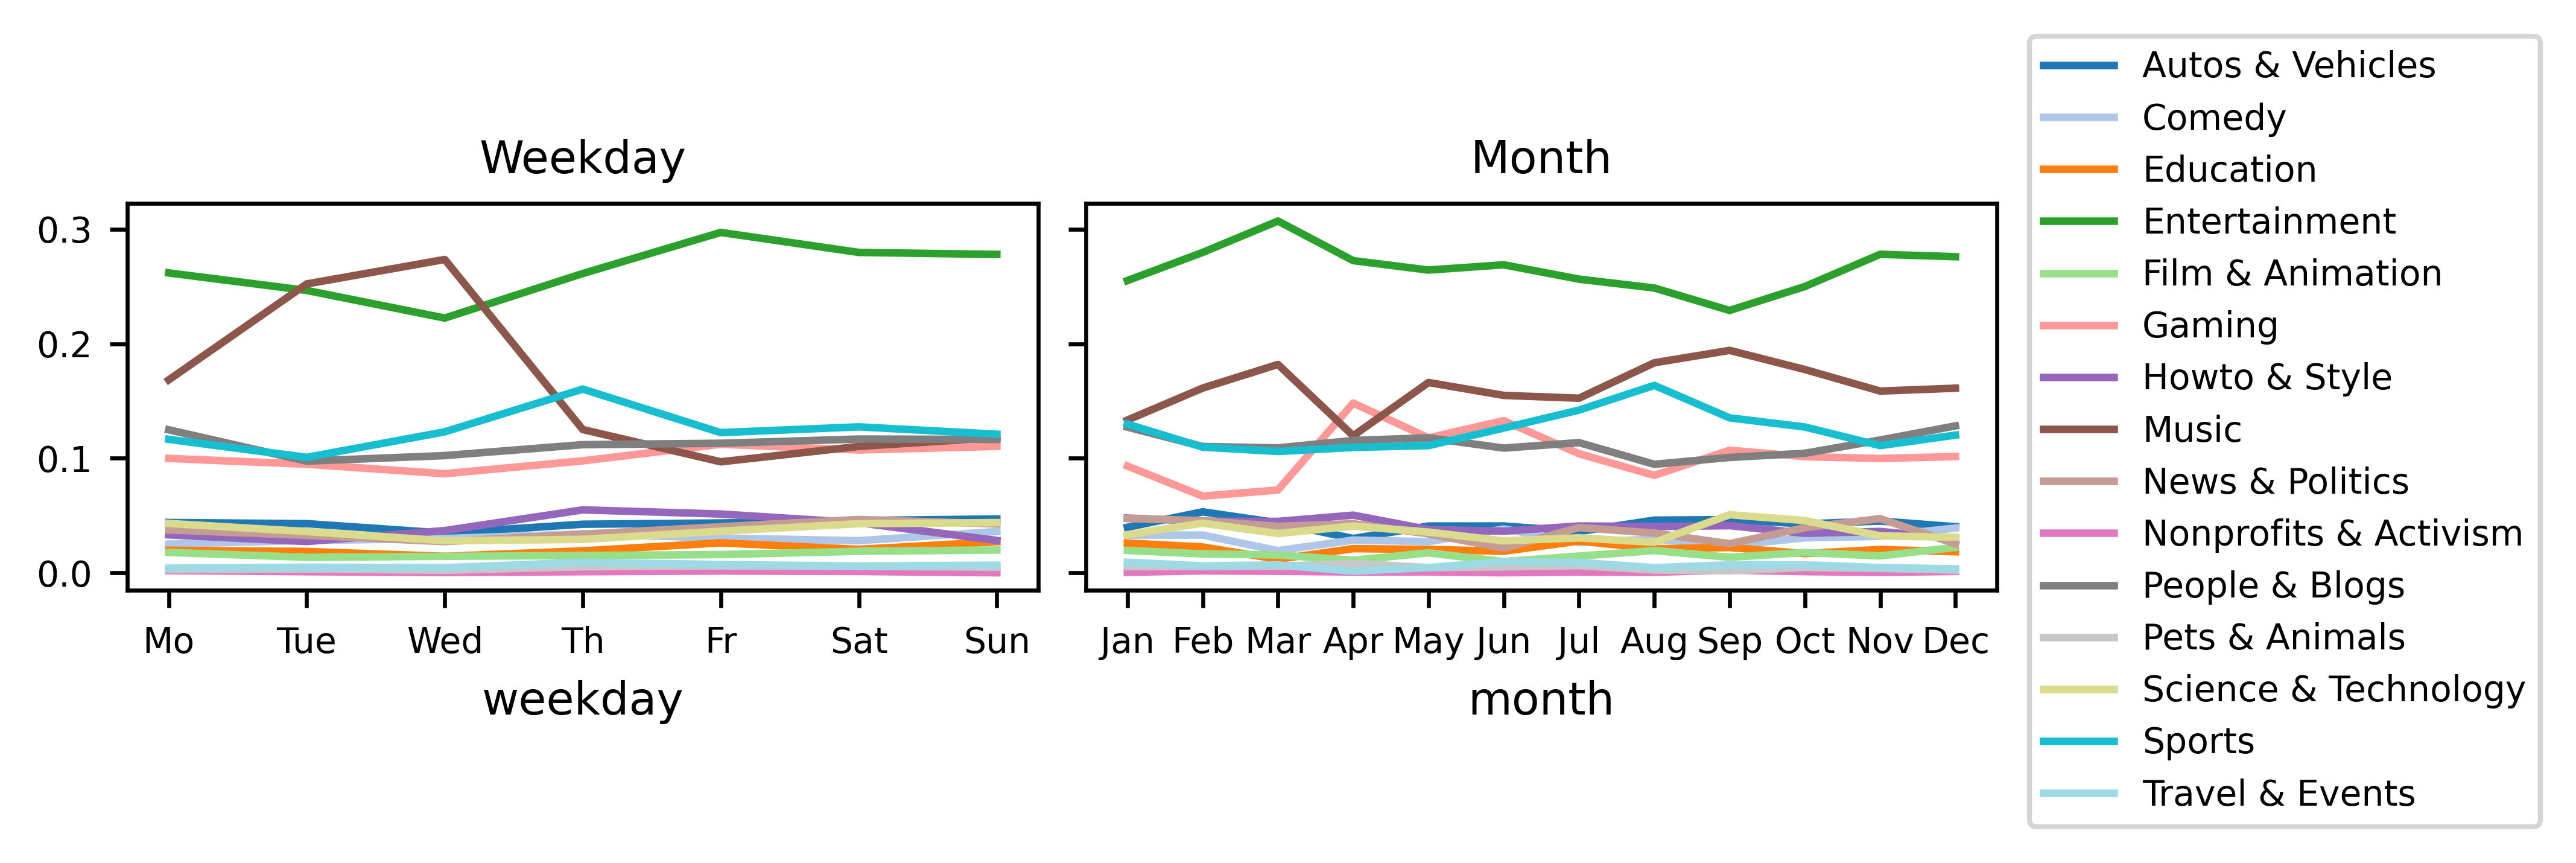
\includegraphics[width=0.9\textwidth]{fig/cat_weekday_month.png}
    \caption{Average share of categories per weekday and month}
    \label{fig:cat_cycle}
\end{figure}
\end{document}
